Before we can start doing anything interesting with our operating system, we need a framework for managing physical memory, since it serves as the backbone of many other OS functions. Physical memory management is done through a structure called the ``memory manager".

\subsection{Capabilities}
Capabilities can be thought of as keys to a door. Under the classical ``access-control" approach to operating systems, different sections of memory are associated with a list of users who have various rights with respect to that section of memory; for example, a file \textbf{F} that can be read from by processes \textbf{A} and \textbf{B}. In contrast, capabilities define a list of memory sections that they have rights to. In terms of our access-control example, processes \textbf{A} and \textbf{B} would instead hold a capability to the file \textbf{F} that allows them to various abilities (read/write/execute) to it. Oftentimes in this paper we will also refer to the ``CSpace", which can simply be thought of as a process' storage for its capabilities. The CSpace is structured as a two-level table that only the kernel may directly modify. When we refer to capabilities in later sections of this report, we really mean a \textit{reference} to the capability, as our user-level processes do not directly manage the capabilities. 

\subsection{Design Constraints}\label{m1-0}
At this stage in our operating system, we have a single, privileged process running, called \texttt{init}. This process has been handed several capabilities to different portions of RAM and we must devise a method through which we can divide and distribute these portions on request. We encapsulate the data structure and algorithm that will perform this task in a ``physical memory manager". From this point forward in our OS, any and all physical memory allocations/frees are performed by this memory manager. Although this memory manager is meant to provide RAM resources to the entire system, as we mentioned earlier, we only have one core running a single process with a single thread. As such, the following sections describe an implementation that does not handle concurrency.
\\\\
The memory manager must keep track of all allocated and free physical memory, otherwise we would not have any way to tell what is and isn't currently being used. When a process requests memory, the memory manager must locate an appropriate section of free physical memory and provide a RAM capability to the caller. RAM capabilities can be understood as just that; capabilities to sections of RAM. They may be retyped into a variety of more fine-grained capabilities (denoting more specific things one might do with the memory that the capability points to), and they also may be passed between processes (the fundamental mechanism by which our memory manager distributes memory).
\\\\
There are two big decisions that need to be made when implementing the memory manager:
\begin{enumerate}[itemsep=0pt]
    \item What data structure should we be using to represent the physical address space? 
    \item Given that we don't know what allocations and frees will happen ahead of time, how do we decide which parts of the physical address space to allocate?
\end{enumerate}
Just as it is when setting out to design any operating system, it was necessary that our group give a lot of thought to these questions as it would have a direct impact on the efficiency of our system in both speed and fragmentation. On that note, however, it should also be mentioned that deadline pressure was a very real factor in the decisions we made; while it would be nice to sit around all day and conjure up hyperefficient implementations of Barrelfish, we sometimes simply didn't have the time to do so. The existence of tight deadlines introduced a few external considerations to our design choices:
\begin{itemize}[itemsep=0pt]
    \item We should reuse code where possible (and reasonable). This saves time in that the code is already verified and doesn't need to be written from the ground up.
    \item Designs should not be overly complicated. Complexity often makes systems more error-prone and causes those errors to take longer to understand/debug.
\end{itemize}
This was especially prevalent for our group considering that we are all full-time students with very different and often clashing schedules. It should become clear over time that these were often some of if not the defining factors in our design decisions.

\subsection{Physical Memory Layout}\label{m1-3}
As mentioned previously, we needed to choose a data structure to maintain metadata regarding the free and allocated regions of physical address space. We also needed our structure to be able to locate appropriate sections of memory to satisfy allocation requests as well as update metadata when regions become free. There were a few considerations that we took into account when choosing such a structure for the memory manager:
\begin{itemize}[itemsep=0pt]
    \item Our data structure should take up an acceptable amount of memory.
    \item We should be able to perform efficient searches through our data structure for given address regions.
    \item We should be able to perform efficient insertions/deletions of address regions using our data structure. We would also ideally like for these operations to not negatively effect subsequent searches through the data structure.
    \item The implementation of our data structure should not be too complex due to the time constraints.
\end{itemize}

\subsubsection{Linked List}\label{m1-2}
We chose to use a linked list to maintain the memory manager's metadata, based on the fact that it provided an acceptable solution with respect to our previous considerations:
\begin{itemize}
    \item A linked list allows us to represent memory regions of arbitrary size and number.
    \item A linked list sacrifices efficient traversal of its nodes for a straightforward, linear-time walk of the list in search for an allocated or free address region. Due to our time constraints, a less complex data structure traversal was of higher value than improved efficiency.
    \item By storing pointers to the next and previous node in the linked list, we can easily insert new nodes or remove nodes at a specific position in our linked list, preserving the order of our list. Although the ordering of nodes in our list is not too important for the physical memory manager, it will play a factor later on in Milestone 2.
\end{itemize}
Nodes of the list represent regions of physical memory and can be either free or allocated. The list contains nodes representing the entire, free address space at the beginning of time. Subsequent operations (such as allocation of a region) split and/or coalesce nodes accordingly. Since nodes represent regions, they also need to store info such as their base address and size. 

\subsection{Allocation Strategy}
An allocation strategy determines which memory region the memory manager chooses to satisfy an allocation request. A good allocation strategy minimizes allocation latency and minimizes fragmentation of the physical address space for an average workload. By ``minimizes fragmentation", we mean that if we have a total X bytes of free memory, ideally we would like to be able to allocate X bytes of memory. In practice however this is nearly never the case due to arbitrary allocation sizes and arbitrary routines of allocations and frees.

\subsubsection{Next Fit}
Out of the memory manager functions we wrote, of particular note is \texttt{choose\_region} which decides what part of the address space to allocate when serving a request. We decided to go with a \texttt{next-fit} strategy here, which chooses the first region suitable for an allocation (it must be free and large enough) and begins its search at the region following whichever one was most previously allocated. For this to work, the memory manager is required to store a pointer to its most recently allocated region and a bit of complexity needs to be added to the algorithm (as compared to something like \texttt{first-fit}), however we decided to go with it nonetheless due to its benefit as a ``jack-of-all-trades" approach.

\subsubsection{Alternative Strategies}
We provide a comparison of \texttt{first-fit}, \texttt{worst-fit}, \texttt{best-fit}, and \texttt{next-fit} (anything more complicated was not considered due to time constraints):
\begin{itemize}[itemsep=-5pt]
    \item \texttt{first-fit}:
    \begin{itemize}[itemsep=0pt]
        \item Simple to implement
        \item Fragments early addresses significantly since we always start at the beginning
        \item Slows down over time as longer walks of the linked list are required
    \end{itemize}
    \item \texttt{worst-fit}:
    \begin{itemize}[itemsep=0pt]
        \item Low fragmentation; keeps large free regions large
        \item Slow, since a full walk is always necessary
    \end{itemize}
    \item \texttt{best-fit}:
    \begin{itemize}[itemsep=0pt]
        \item Minimizes external fragmentation
        \item Slow, since a full walk is always necessary 
    \end{itemize}
    \item \texttt{next-fit}:
    \begin{itemize}[itemsep=0pt]
        \item Reasonable fragmentation (spreads allocations across the space)
        \item Reasonably fast; searches finish quicker since we remember where we stopped
    \end{itemize}
\end{itemize}
We compared \texttt{first-fit} and \texttt{next-fit} in the case of many subsequent allocations without any frees (Figure \ref{figure:mm_alloc_scatter}) and found that both appear to demonstrate linear growth in latency with respect to the number of allocated regions, however \texttt{next-fit} grows more slowly. Upon choosing an appropriate RAM capability, the memory manager must split and retype it to return to the requesting process. Retyping a capability must be handled with care, so as to not fall into a case where a region of physical memory is referred to by capabilities of conflicting types, and thus require walking of the process's CSpace to check for descendants or siblings of the capability. Due to this retyping operation, which approximately requires linear time, it is not possible to have sub-linear growth in either \texttt{first-fit} or \texttt{next-fit}. Note that there appears to be a second, lower-density line of higher-latency points; these likely correspond to allocations that triggered slab/slot allocator refills (detailed in the next section).
\begin{figure}[ht]
    \centering
    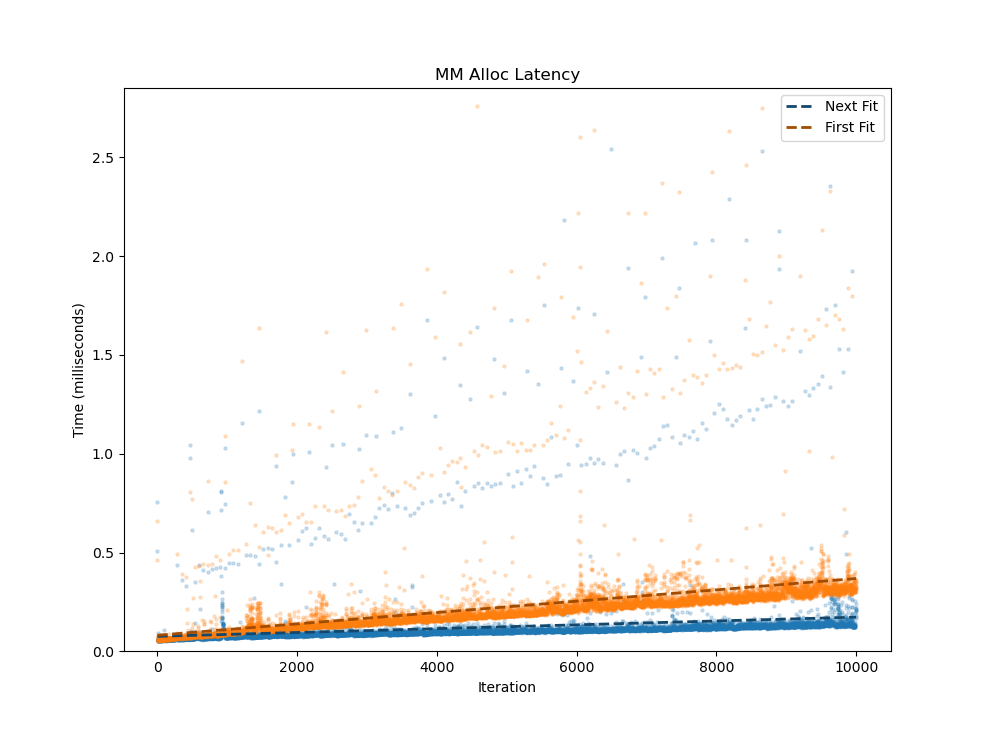
\includegraphics[width=\columnwidth]{images/mm_alloc_scatter.png}
    \caption{Allocation latencies for different strategies.}
    \label{figure:mm_alloc_scatter}
\end{figure}

\subsection{Allocator Refills}
Since the memory manager cannot dynamically allocate memory to store data in, it uses ``slab allocators" to partition memory into small chunks for storage of its metadata nodes. It also uses a ``slot allocator" which allocates capability slots from the CSpace such that the memory manager can store new retyped capabilities (remember, capabilities themselves take up memory). Both of these allocators occasionally require memory refills which are served by the memory manager.
\\\\
To prevent an infinite loop of allocator refills, we set a \texttt{refill} flag whenever an allocator initiates a refill. Until the flag is cleared, no refills are to be triggered. To ensure that there are enough remaining resources to fully complete a refill request, slot and slab allocators have a respective thresholds. When the number of slots/slabs dips below the threshold, a refill is triggered. 

\subsection{Alternative Memory Manager Designs}\label{m1-6}
A disadvantage of linked lists is that finding a particular region takes time $O(n)$ for $n$ nodes. This is particularly relevant when freeing a region, since it first needs to be located in the list.
\\\\
We considered a few alternative data structures:
\begin{itemize}[itemsep=0pt]
        \item \texttt{Static array}: This looks good at first glance on basis of lookups and insertions being constant-time, however using a static array would either severely limit the number of possible allocations, or introduce a massive memory overhead.
        \item \texttt{Balanced tree}: A more complex data structure such as a balanced binary search tree might provide faster lookup times. If the tree is sorted by address, it would allow freeing a region in $O(logn)$ rather than the $O(n)$ for a linked list. Depending on the allocation strategy, the tree might better be sorted by region size which would support a fast implementation of best-fit or worst-fit. However, more complex data structures are also most prone to errors. Since bugs in the memory manager could severely impact all other aspects of the system, we chose to avoid a complex implementation like this. 
\end{itemize}

\subsection{Partial Frees}
We chose to implement partial frees, allowing a procedure to free only a subset of an originally allocated address region. Luckily, the linked-list data structure allowed us to implement this easily through splitting of an allocated region's node in the linked list and marking only the requested segment as free.

\subsection{Ranged Allocation}
We also chose to implement ranged allocations, allowing procedures to make allocation requests within a specified region of physical addresses. Since the linked list maintains address order it also wasn't too tough to implement this; we walk the list and search for any regions containing addresses within the requested range which have a sufficient size. If one is found it can be split appropriately and only the requested region will be marked as allocated.
